\vspace{10pt}

{\centering\subsection*{贺帅:她后悔了}}

\addcontentsline{toc}{subsection}{贺帅:她后悔了}

\renewcommand{\leftmark}{贺帅:她后悔了}

\begin{figure}[htbp]

\centering

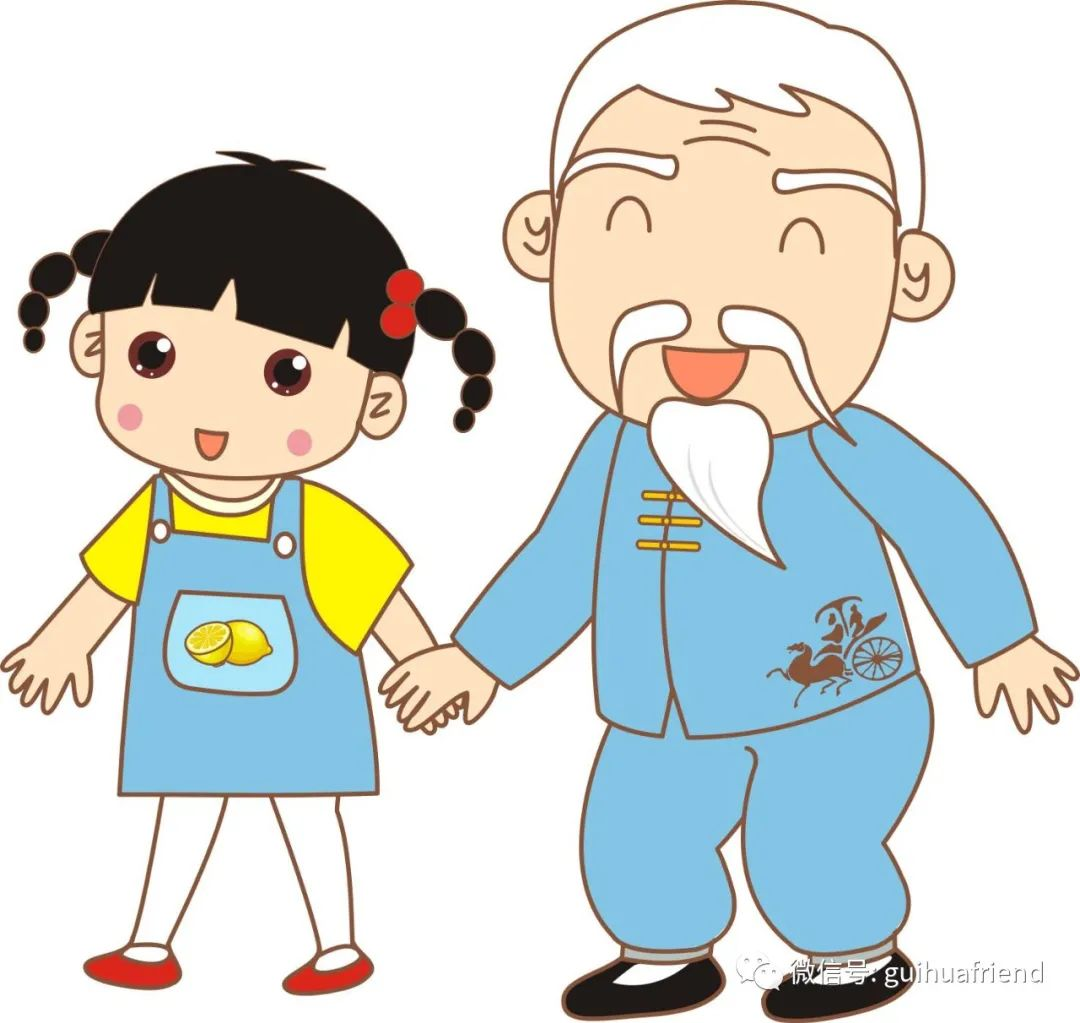
\includegraphics[width = .5\textwidth]{./ch/39.jpg}

\end{figure}



每个人的心情都会变化多端,有时开心,有时悲伤,有时高兴,有时失望,有时是因为考了个非常棒的分数而高兴,有时是因为被家人教训而悲伤,还有时是因为朋友没答应自己的事情而失望。因为这件事她非常后悔。在安静的书房里,小丽正在开心地看着故事书,看得正起劲的时候,突然爷爷说了一句话:“小丽,小丽这台电视怎么播节目呢?”小丽被吵得不耐烦了,急忙跑出去对爷爷说:“爷爷,你怎么连这么简单的设备都不会用,你不会就不要看了吧!"顿时,爷爷转过头去悄悄地抹着眼泪。小丽看到爷爷脸上的泪水,非常难过,他不知道该怎么办,就急忙跑回书房。过了好一会儿,小丽怎么也静不下心来看书,她想去找爷爷道歉,可他又怕太尴尬,迟迟不敢去。又过了一会儿,小丽真的忍不住了,她心里想:“爷爷平时对我这么好,把好吃好喝好玩的东西都给我,而我却总是让爷爷失望,我真的太对不起爷爷。”可她还是不敢,她想等爷爷走过来时再和爷爷道歉。可等来等去爷爷都没有走过来,她知道必须要自己去主动找爷爷道歉,她一边捶着自己的胸口一边说:“如果我不去,爷爷会非常失望,我不配做他的孙女。”说到这里,小丽终于忍不住了,她一边哭着一边跑出去对爷爷说:“爷爷,对不起,我不应该凶你的,我答应您以后再也不凶您了。”爷爷的脸上又露出了慈祥的表情。如果每个人都献出一点爱心,整个世界就永远会是光明的。



\vspace{10pt}



作者:五(2)班 贺帅

指导老师:周璇

投稿:2021年4月15日

发表:2021年4月22日


                



\vspace{10pt}

\hline



